\subsection{Setup}
All experiments use the \texttt{exp} configuration: $d_{\mathrm{model}}=128$, 4
layers in an \texttt{MMA} layout (3 Mamba-2 + 1 attention), 7.67M parameters in
total with the tied GPT-2 BPE vocabulary (50,257). Training data is a
single-domain Chinese technical corpus of 8,492 tokens (6,112 UTF-8 characters),
split 95/5 into train/validation. Each sequence has length 128; batch size is 8
with 2 gradient-accumulation steps (effective batch 16); the peak learning rate
is $10^{-3}$ with warmup and cosine decay; precision is bf16 mixed precision on
a 2-core CPU with oneDNN. All runs use seed 42 and 400 optimization steps.

The baseline and drive-enabled runs are identical except that the latter adds
the drive-signal layer ($w_{\mathrm{reg}}=0.01$,
$w_{\mathrm{desire}}=0.5$, $w_{\mathrm{fear}}=1.0$; setpoints and target state
as described in Section~\ref{sec:drives}).

\subsection{Pretraining: baseline versus drive-enabled}
Figure~\ref{fig:loss} shows the training loss curves. Both runs converge
rapidly on the small corpus (training perplexity approaches $\sim$1, indicating
overfitting, which is expected at this scale). The drive-enabled run maintains
a slightly higher training loss throughout, which is the expected effect of the
regularization term $\mathcal{L}_{\mathrm{drive}}$: the model trades a small
amount of training fit for a better-controlled optimization trajectory.

\begin{figure}[t]
  \centering
  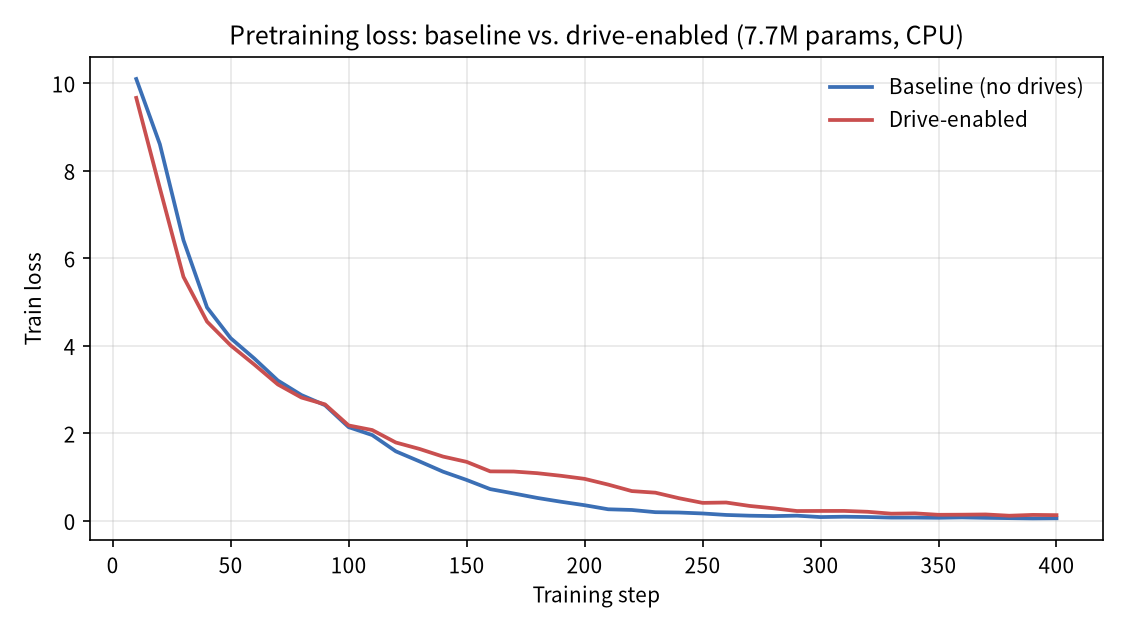
\includegraphics[width=0.92\linewidth]{figs/loss_curve.png}
  \caption{Pretraining loss curves (train). The drive-enabled run carries a
  small loss overhead from the drive regularization term.}
  \label{fig:loss}
\end{figure}

Crucially, the drive-enabled model achieves a \emph{better} validation
perplexity: $2.463$ (PPL $11.74$) versus $2.616$ (PPL $13.68$) for the
baseline --- a relative improvement of $5.9\%$ in validation loss. This
indicates that the homeostatic drive layer, far from hurting training, acts as
an effective regularizer that improves generalization in this setting
(Figure~\ref{fig:val}).

\begin{figure}[t]
  \centering
  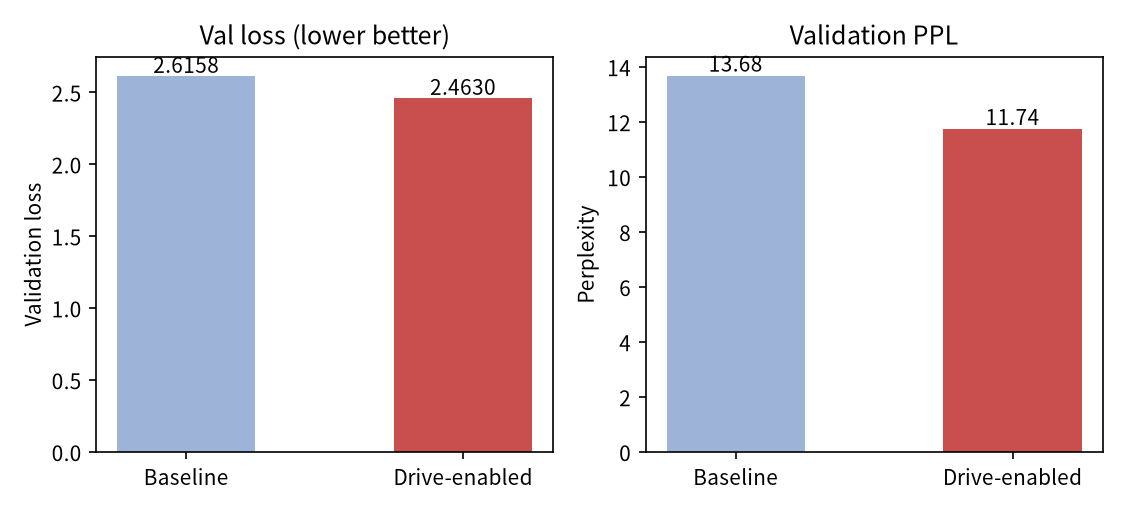
\includegraphics[width=0.92\linewidth]{figs/val_compare.png}
  \caption{Validation loss and perplexity at the end of training.}
  \label{fig:val}
\end{figure}

\subsection{Dynamics of the drive signals}
Figure~\ref{fig:drives} plots the internal state and derived signals during the
drive-enabled run. Several observations are of note:
\begin{itemize}
  \item \textbf{Energy} depletes monotonically from its setpoint (0.8) to 0 as
  training consumes the compute budget; the rate-limited update keeps the
  trajectory smooth.
  \item \textbf{Deviation} $D$ rises from $\sim$0.12 to a steady $\sim$0.44--0.51
  as components leave their setpoints, and \textbf{desire} tracks it closely,
  indicating a persistent ``wanting'' of the target state.
  \item \textbf{Fear} remains 0 throughout: the model never projects outside the
  safety boundary, i.e., the drive layer keeps the system ``homeostatically
  safe'' as designed. Consequently the learning-rate brake is never engaged.
  \item \textbf{Consistency} grows toward the end of training as the loss
  variance shrinks, matching its semantic (stability of recent outputs).
\end{itemize}

\begin{figure}[t]
  \centering
  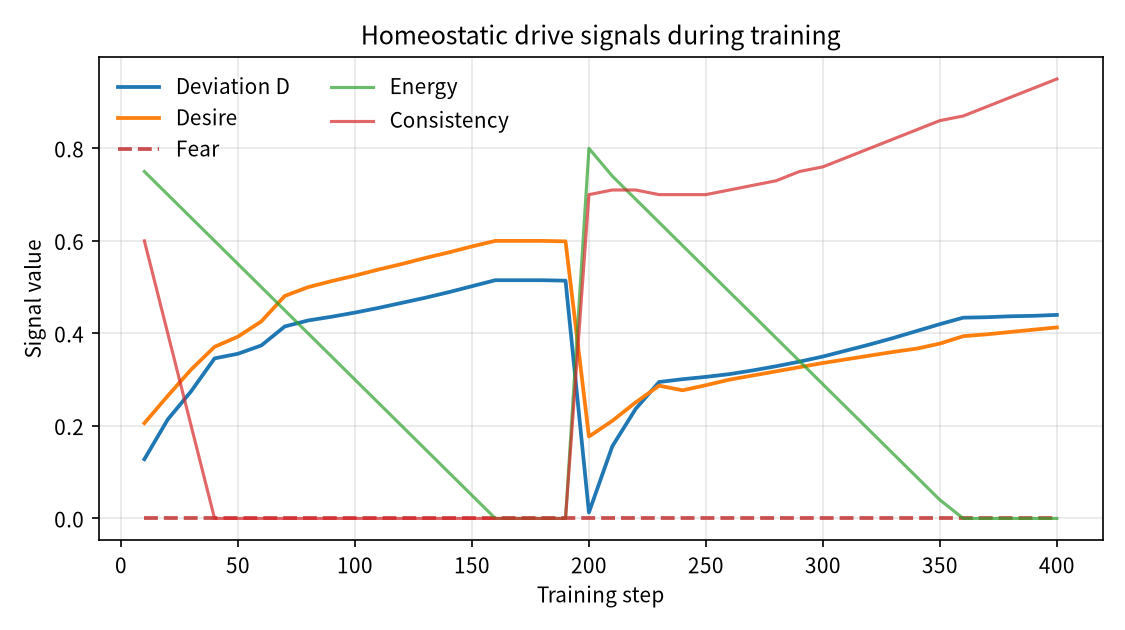
\includegraphics[width=0.92\linewidth]{figs/drive_signals.png}
  \caption{Drive-signal dynamics during the drive-enabled run. Energy depletes,
  deviation and desire rise to a steady state, fear stays at zero (no
  safety-boundary violation), and consistency grows as training stabilizes.}
  \label{fig:drives}
\end{figure}

\subsection{SFT, DPO, and generation}
Starting from the baseline pretrained checkpoint, supervised fine-tuning on the
12-example instruction set drives the SFT loss from $\sim$4.0 to $0.28$ in 200
steps. Direct preference optimization on the 8-pair preference set further
reduces the DPO loss to $0.047$ in 150 steps with a frozen reference model. Both
stages run in a few minutes on CPU and confirm that the full
pretrain$\rightarrow$SFT$\rightarrow$DPO pipeline is operational.

We note honestly that generation quality at this scale is limited: with 7.67M
parameters, a Chinese corpus of only 8k tokens, and an English-oriented
byte-pair tokenizer, sampled outputs are fragmentary (short Chinese n-grams
with occasional incoherence). This is a documented limitation of tiny models on
tiny corpora rather than a defect of the pipeline, and we report it as such.
Larger corpora, a Chinese-optimized tokenizer, and more parameters are required
for fluent generation; the current experiments validate the \emph{mechanisms}
(training dynamics, alignment, and drive control) rather than end-task quality.
